\documentclass[12pt,a4paper]{article}

% --------------------
% Paquetes necesarios
% --------------------
\usepackage[spanish]{babel}     
\usepackage[utf8]{inputenc}     
\usepackage[T1]{fontenc}        
\usepackage{fancyhdr}           
\usepackage{hyperref}           
\usepackage{graphicx}           

% --------------------
% Información del trabajo
% --------------------
\newcommand{\miNombre}{Pedro González Fernández}
\newcommand{\miAsignatura}{Sistemas de Big Data}
\newcommand{\tituloTrabajo}{Falacias en Gráficos}

% --------------------
% Configuración de encabezado/pie
% --------------------
\pagestyle{fancy}
\fancyhf{}
\fancyhead[L]{\miNombre}
\fancyhead[R]{\miAsignatura}
\fancyfoot[C]{\thepage}

% --------------------
% Título del documento
% --------------------
\title{\tituloTrabajo}
\author{\miNombre}
\date{\today}

% --------------------
% Documento
% --------------------
\begin{document}

\maketitle
\begin{figure}[h]
    \centering
    \includegraphics[width=0.7\textwidth]{falacia.png}
    \label{fig:portada}
\end{figure}

\tableofcontents
\newpage

% --------------------
% Contenido
% --------------------
\section{Enunciado}
En este trabajo se presentan dos gráficos con falacias visuales y dos con falacias relacionales. 
En cada caso se explica en qué consiste la falacia y cómo afecta a la interpretación de los datos.

\section{Desarrollo}

\subsection{Falacias Visuales}
Una \textbf{falacia visual} es una representación gráfica que induce a error mediante recursos puramente visuales, 
como escalas alteradas, proporciones engañosas o diseños que distorsionan la percepción.

\subsubsection{Variación del precio de la luz en España}
\begin{figure}[h]
    \centering
    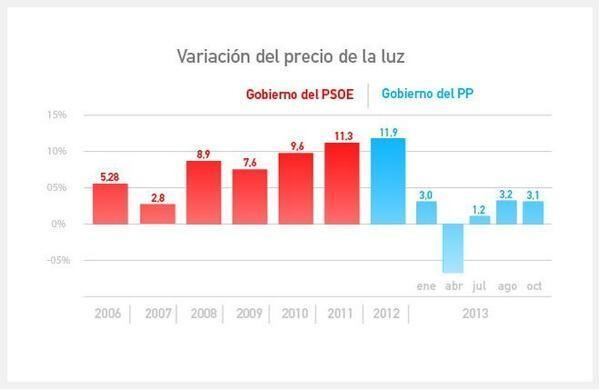
\includegraphics[width=0.7\textwidth]{falacia2.jpg}
    \caption{Variación del precio de la luz en España.}
    \label{fig:grafico2}
\end{figure}
Este gráfico muestra la evolución del precio de la luz entre 2006 y 2013. 
El problema surge en 2013, cuando se \textbf{cambia la escala temporal de anual a trimestral}. 
Este cambio induce a pensar que el \textbf{precio bajó bruscamente}, cuando en realidad se están comparando periodos de distinta duración.

\newpage

\subsubsection{Diferencia de puntos en LaLiga}
\begin{figure}[h]
    \centering
    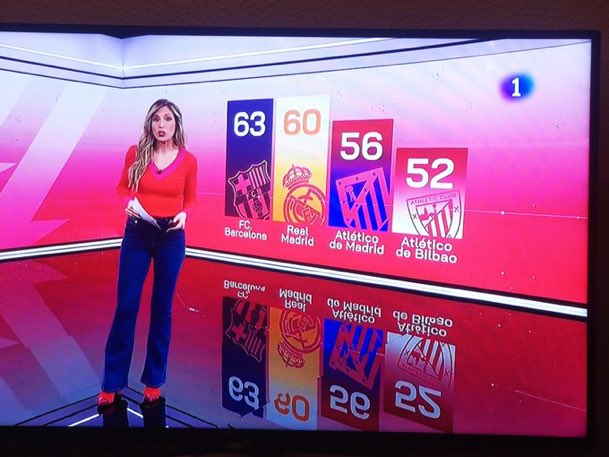
\includegraphics[width=0.7\textwidth]{falacia3.jpg}
    \caption{Diferencia de puntos entre los 4 primeros de LaLiga.}
    \label{fig:grafico3}
\end{figure}
Aquí se comparan los puntos de los cuatro primeros equipos de LaLiga. 
Aunque la diferencia entre Barcelona y Real Madrid es de 3 puntos, \textbf{sus barras aparecen iguales}. 
En cambio, la diferencia de 4 puntos entre Atlético y Athletic se representa con \textbf{barras mucho más desiguales}. 
Esto genera una \textbf{percepción errónea de las diferencias reales}.

\newpage

\subsection{Falacias Relacionales}
Las \textbf{falacias relacionales} ocurren cuando los datos son correctos, 
pero la relación establecida entre variables lleva a interpretaciones equivocadas. 
Esto suele deberse a correlaciones sin sentido o comparaciones inadecuadas.

\subsubsection{Consumo de mozzarella vs. graduados en Ingeniería Civil}
\begin{figure}[h]
    \centering
    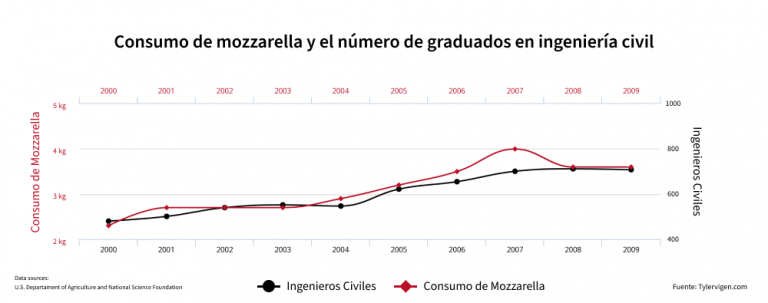
\includegraphics[width=0.7\textwidth]{falacia1.png}
    \caption{Consumo de mozzarella vs. graduados en Ingeniería civil.}
    \label{fig:grafico1}
\end{figure}
El gráfico sugiere una correlación entre \textbf{consumo de mozzarella y número de graduados en ingeniería civil} en EE.UU. 
Aunque ambas variables aumentan, no existe \textbf{relación causal}. 
La asociación \textbf{carece de sentido} y probablemente se deba a \textbf{factores externos} como el crecimiento poblacional.

\subsubsection{Abandono de perros por comunidad autónoma}
\begin{figure}[h]
    \centering
    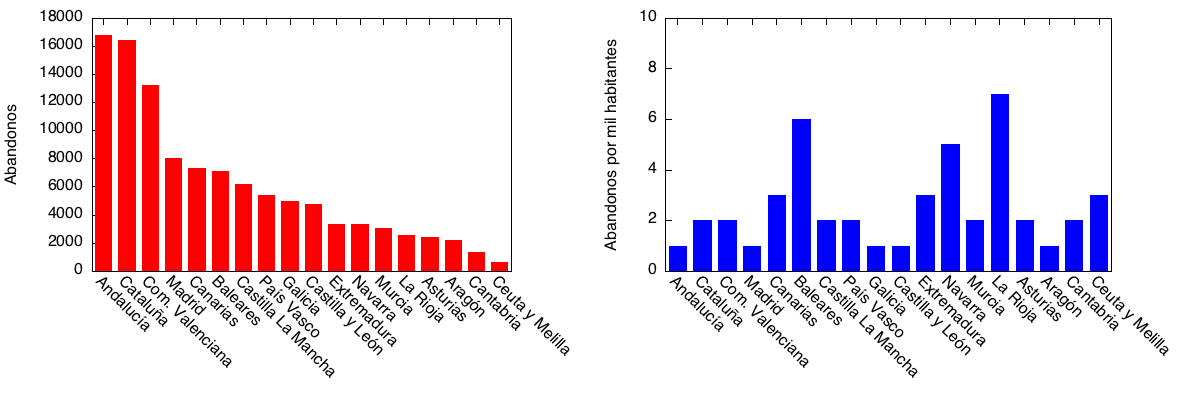
\includegraphics[width=0.7\textwidth]{falacia4.png}
    \caption{Abandono de perros por comunidad autónoma.}
    \label{fig:grafico4}
\end{figure}
El gráfico de la izquierda muestra abandonos absolutos de perros por comunidad. 
Esto da la impresión de que \textbf{Andalucía y Cataluña son las peores}, pero también son las \textbf{más pobladas}. 
El gráfico de la derecha ajusta por \textbf{cada mil habitantes}, mostrando que en realidad comunidades pequeñas como \textbf{La Rioja o Baleares presentan más abandonos en proporción}.

\end{document}
